% latex svg-output-example; dvisvgm svg-output-example
\documentclass[border=10pt]{standalone}
\usepackage{tikz}
\usetikzlibrary{intersections}

\begin{document}
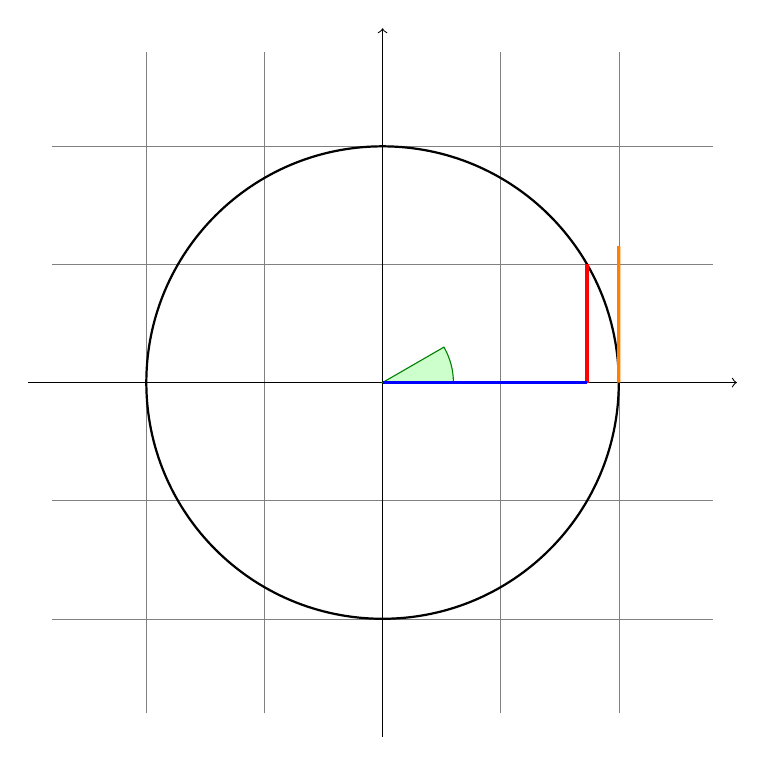
\begin{tikzpicture}[scale=3]
    % \path[draw,clip] (0.25,0.25) circle (0.75cm);
    
    \draw[step=.5cm,gray,very thin] (-1.4,-1.4) grid (1.4,1.4); 
    \draw[->] (-1.5,0) -- (1.5,0);
    \draw[->] (0,-1.5) -- (0,1.5);
    \draw[thick] (0,0) circle [radius=1cm];

    \filldraw[fill=green!20, draw=green!50!black] 
        (0,0) -- (3mm,0mm) arc [start angle=0,end angle=30,radius=3mm] -- cycle;
    
    \draw[red,very thick] (30:1cm) -- (30:1cm|-0,0);
    \draw[blue,very thick] (30:1cm|-0,0) -- (0,0);

    % to find tan(30) "geometrically", as an intersection of two lines:
    \path [name path=upward line] (1,0) -- (1,1);
    % a bit longer, so that there is an intersection:
    \path [name path=sloped line] (0,0) -- (30:1.5cm); 
    % (add `\usetikzlibrary{intersections}' after loading tikz in the preamble)
    \draw [name intersections={of=upward line and sloped line, by=x}] 
          [very thick,orange] (1,0) -- (x);

\end{tikzpicture}
\end{document}